\documentclass[9pt]{extarticle}

% ---------- Build padding ----------
% The build script passes a blank-page count so the print run ends on a whole
% sheet, whatever the binding.
\providecommand{\buildpad}{0}

% ---------- Page geometry: A6, 105 x 148 mm ----------
% The inner margin carries the binder's gutter; the outer stays narrow so the
% text block keeps its width on a page this small.
\usepackage[twoside,paperwidth=105mm,paperheight=148mm,
            top=11mm,bottom=13mm,inner=12mm,outer=8mm]{geometry}

% ---------- Fonts ----------
\usepackage{fontspec}
\setmainfont{TeX Gyre Pagella}
\usepackage{microtype}
\usepackage{titlesec}
\usepackage{needspace}
\usepackage{graphicx}
\usepackage{etoolbox}
\usepackage{fancyhdr}
\usepackage{pifont}
\usepackage{marvosym}

% ---------- Section heading styling ----------
\titleformat{\section}
  {\centering\normalfont\large\bfseries\scshape\addfontfeature{LetterSpace=8}}
  {}{0pt}{}[\thispagestyle{plain}]
\titlespacing*{\section}{0pt}{0pt}{1.0em}
\setcounter{secnumdepth}{0}
\setcounter{tocdepth}{1}

% ---------- Footnote styling ----------
\renewcommand{\footnotesize}{\fontsize{7.5}{9}\selectfont}
\renewcommand{\thefootnote}{\Cross}

% ---------- Dotted leaders in the contents ----------
\usepackage[hidelinks,bookmarks=true,bookmarksopen=false]{hyperref}
\makeatletter
\patchcmd\l@section{%
  \nobreak\hfil\nobreak
}{%
  \nobreak
  \leaders\hbox{%
    $\m@th \mkern \@dotsep mu\hbox{.}\mkern \@dotsep mu$%
  }%
  \hfill
  \nobreak
}{}{\errmessage{\noexpand\l@section could not be patched}}
\patchcmd{\l@section}{\addvspace{1.0em \@plus\p@}}{\addvspace{0.2em \@plus\p@}}{}{}
% in-text footnote mark and footer mark: a cross
\renewcommand{\@makefnmark}{\textsuperscript{\Cross}}
\renewcommand{\@makefntext}[1]{%
  \parindent 1em\noindent
  \hb@xt@1.8em{\hss\Cross\enspace}#1}
\makeatother

\setlength{\parindent}{0pt}
\setlength{\parskip}{0pt}
\setlength{\emergencystretch}{3em}
% do not open or close a paragraph with a single line
\widowpenalty=10000
\clubpenalty=10000

\setlength{\headheight}{12pt}
\setlength{\headsep}{8pt}
\pagestyle{fancy}
\fancyhf{}
\fancyhead[C]{\footnotesize\scshape\leftmark}
\fancyfoot[C]{\footnotesize\thepage}
\renewcommand{\headrulewidth}{0pt}
\fancypagestyle{plain}{\fancyhf{}\fancyfoot[C]{\footnotesize\thepage}\renewcommand{\headrulewidth}{0pt}}

\begin{document}

% Common formatting commands.
% The book is printed in one ink, so hierarchy is carried by size, weight and
% small caps. Colour used to mark rubrics and prayer titles, and without it a
% black italic line is easily mistaken for prayer text, so rubrics drop a step
% in size and prayer titles take the bold face.

% heading face: bold small caps, letter-spaced
\newcommand{\headingfont}{\bfseries\scshape\addfontfeature{LetterSpace=6}}

% rubric / instruction text, a step down from the body. The reserve keeps the
% rubric with the first lines of what it introduces; without it a rubric can be
% left alone at the foot of a page.
\newcommand{\rubricsize}{\fontsize{8.5}{10.5}\selectfont}
\newcommand{\rubric}[1]{{\rubricsize\itshape #1}}
\newcommand{\rubricline}[1]{\par\vspace{0.6em}\rubric{#1}\par\vspace{0.3em}}
\newcommand{\instruction}[1]{\needspace{5\baselineskip}\rubricline{#1}}
% a rubric that introduces a prayer title: reserve for the rubric and for the
% title's own reserve, so the two never part company across a page break
\newcommand{\instructionheading}[1]{\needspace{11\baselineskip}\rubricline{#1}}
% a rubric that closes a block of prayer. Nothing follows that it must stay
% with, so it reserves its own line alone and may sit at the foot of a page.
\newcommand{\instructionclosing}[1]{\needspace{2\baselineskip}\rubricline{#1}}

% label over a prayer, kept with the text it introduces
\newcommand{\theotokion}{\needspace{5\baselineskip}{\headingfont Theotokion}}

% a division inside the canon of preparation: an ode number, or the kontakion
\newcommand{\canonlabel}[1]{\needspace{6\baselineskip}\par\vspace{0.8em}\begin{center}{\headingfont\normalsize #1}\end{center}}

% prayer title heading, centred
\newcommand{\prayer}[1]{\needspace{8\baselineskip}\par\vspace{0.3em}\begin{center}{\headingfont\normalsize #1}\end{center}}

\newcommand{\refrain}[1]{\par\vspace{0.4em}\textit{#1}\par\vspace{0.4em}}

% ornamental rule: line, star, line. The optional argument is the fraction of
% the text width taken by each line, so a flair can be matched to what it frames.
% It is set as one line of a paragraph rather than inside a center environment:
% a list injects its own breakpoint, which lets the rule be torn away from the
% text it should close.
\newcommand{\ornarule}[1][0.28]{%
  \par\noindent\hspace*{\fill}%
  \rule{#1\textwidth}{0.4pt}\raisebox{-2.58pt}{\,\footnotesize \ding{85}\,}\rule{#1\textwidth}{0.4pt}%
  \hspace*{\fill}\par
}

% A plume over a circle with a leaf either side, drawn upward from a rule. The
% bristles start inside the circle rather than at its crown, so they read as
% coming out of it, and the leaves sweep away from behind it. The leaf teeth are
% points on the leaf's own outline, so no stroke ends float free.
% #1 is the coordinate where it sits on the rule.
\newcommand{\plumeornament}[1]{%
  \begin{scope}[shift={(#1)}]
    \foreach \sx in {1, -1}{%
      \draw[line width=0.4pt, xscale=\sx, yshift=-0.9mm]
        (0.31mm,0.55mm) -- (1.00mm,0.79mm) -- (1.53mm,1.52mm) -- (2.40mm,1.43mm)
        -- (2.98mm,2.03mm) -- (3.89mm,1.93mm) -- (4.56mm,2.33mm) -- (5.39mm,2.41mm)
        -- (5.75mm,2.54mm) -- (5.47mm,2.28mm) -- (4.94mm,1.61mm) -- (4.21mm,1.29mm)
        -- (3.67mm,0.51mm) -- (2.80mm,0.48mm) -- (2.21mm,-0.21mm) -- (1.29mm,-0.01mm)
        -- (0.58mm,-0.27mm) -- cycle;}
    \draw[line width=0.4pt] (0,0) -- (0,1.2mm);
    \draw[line width=0.4pt] (0,2.6mm) circle (1.4mm);
    \begin{scope}[shift={(0,2.6mm)}]
      \foreach \a in {30, 45, ..., 150}{%
        \draw[line width=0.3pt] (\a:1.0mm)
          -- (\a:{1.0mm+2.3mm*(0.86+0.14*cos(\a-90))});}
    \end{scope}
  \end{scope}
}
% the same rule, printed only if the page has room for it. Used to close the
% book: a decoration must not push the run onto another page, nor be left alone
% on a page of its own, so where there is no room it is simply not printed.
\newcommand{\ornaruleiffits}[1][0.28]{%
  \ifdim\pagegoal<\maxdimen
    \ifdim\dimexpr\pagegoal-\pagetotal\relax>2.5\baselineskip
      \vspace{1em}%
      \ornarule[#1]%
    \fi
  \fi
}

\input{commands/prayers.tex}

% Title page
\thispagestyle{empty}
% pull the foot of the page up, so the year below sits well clear of the trim
\enlargethispage{-24mm}
\begin{center}
\vspace*{26mm}
{\scshape\LARGE\addfontfeature{LetterSpace=6} Little Red Prayer Book}

\vspace{8mm}
\ornarule
\vspace{8mm}

{\scshape\normalsize St Andrew's Orthodox Community}\\[2pt]
{\scshape\normalsize Edinburgh}

% the year sits near the foot of the page
\vfill
{\scshape\normalsize 2026}
\end{center}

\newpage

% Icon of Saint Andrew the First-Called: no title, centred, between a top rule
% carrying a thistle and a plain bottom rule. The emblem is Scotland's, whose
% patron he is. Rules, thistle and icon are one picture, so they need no overlay
% pass to line up. No rule runs down either side.
\thispagestyle{empty}
\vspace*{\fill}
\begin{center}
\begin{tikzpicture}
  \node[inner sep=0pt] (icon) {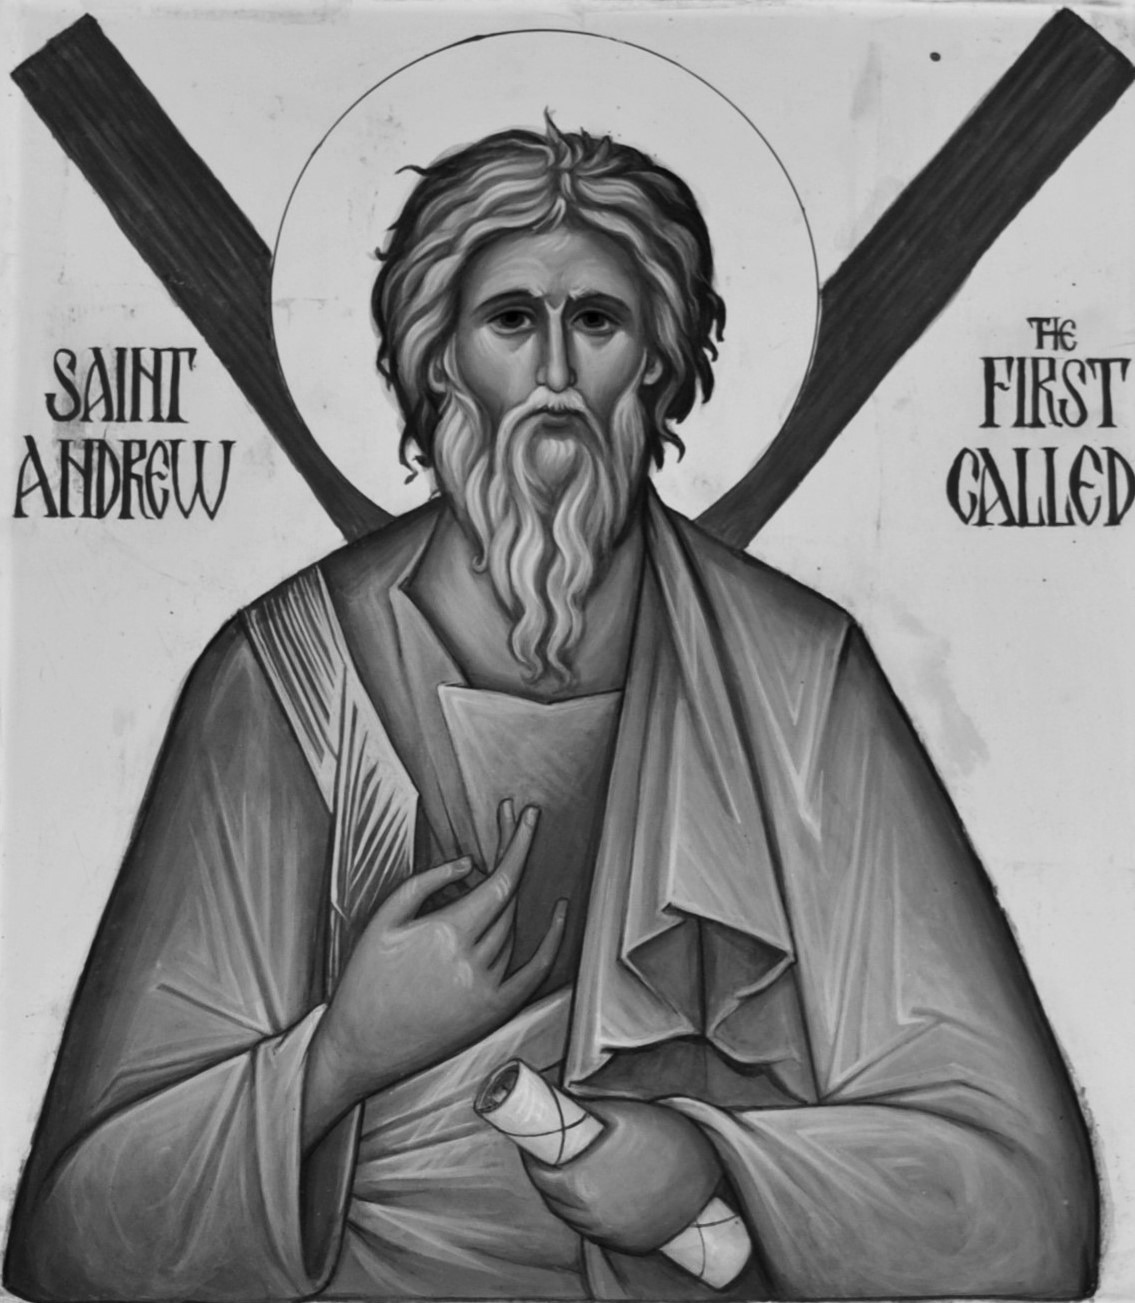
\includegraphics[width=68mm]{assets/icon.jpg}};

  \draw[line width=0.5pt] ([shift={(-4mm,4mm)}]icon.north west)
    -- ([shift={(4mm,4mm)}]icon.north east);
  \draw[line width=0.5pt] ([shift={(-4mm,-4mm)}]icon.south west)
    -- ([shift={(4mm,-4mm)}]icon.south east);

  \coordinate (ornament) at ([shift={(0,4mm)}]icon.north);
  \plumeornament{ornament}
\end{tikzpicture}
\end{center}
\vspace*{\fill}
\newpage


{\small\tableofcontents}
\thispagestyle{plain}
\newpage

% paragraph spacing for the prayer services
\setlength{\parskip}{3pt}

\newpage
% Morning Prayers
\section{Morning Prayers}

\throughtheprayers

\heavenlyking\footnote{\rubric{The prayer,} \textbf{Heavenly King} \rubric{is not said from Pascha until Pentecost. From Pascha until Leavetaking, instead say} \textbf{Christ is risen from the dead...} \rubric{three times.}}

\prayer{The Trisagion Prayers}

\trisagion

\prayer{Hymns to the Trinity}

\instruction{Tone 1}

On rising from sleep, we fall down before you, O Good One, and we cry to you with the Angels' hymn, O Mighty One: Holy, Holy, Holy are you, O God; through the Mother of God have mercy on us.

\refrain{\glory.}

\instruction{Tone 2}

You have roused me, Lord, from my bed and from sleep; enlighten my mind and open my heart and my lips to hymn you, O Holy Trinity: Holy, Holy, Holy are you, O God. Through the Mother of God have mercy on us.

\refrain{\bothnow}

\instruction{Tone 3}

The Judge will come suddenly, and the deeds of each will be laid bare; but with fear let us cry to you in the middle of the night: Holy, Holy, Holy are you, O God. Through the Mother of God have mercy on us.

\mercy{12}

\prayer{Psalm 120}

\psalmonetwenty

\glorybothnow

\prayer{The Symbol of Faith}

\creed

\prayer{Prayer of Thanksgiving with Intercession}

Having risen from sleep I thank you, O Holy Trinity, because through your great goodness and patience you have not been angry with me, an idler and a sinner, nor have you destroyed me in my iniquities, but have shown your customary love for humankind and roused me, as I lay in despair, to rise before dawn and to glorify your might. And now, enlighten the eyes of my mind and open my mouth to meditate on your words, to understand your commandments and to do your will, and to sing to you with a grateful heart and to hymn your all-holy name, of Father, Son and Holy Spirit, now and for ever, and to the ages of ages. Amen.

\prayer{Another Prayer}

Glory to you, O King, almighty God, because in your divine providence and love for humankind you have permitted me, sinner and unworthy, to rise from sleep and to gain entrance to your holy house. Accept, too, Lord, the voice even of my supplication, as you do that of your holy and spiritual Powers, and be well pleased for praise to be offered you with a pure heart and a spirit of humility from my sordid lips, that I too may become a companion of the prudent virgins with the shining lamp of my soul and may glorify you, God the Word, who are glorified with the Father and the Spirit. Amen.

\prayer{Prayer of Saint Basil the Great}

\instruction{Said daily, except on Saturdays}

We bless you, most high God and Lord of mercy, who ever do with us great and unfathomable things, things glorious and extraordinary without number, who have granted us sleep for the refreshment of our weakness and relaxation from the toils of our much-wearied flesh. We thank you that you have not destroyed us in our iniquities, but have shown your customary love for humankind and raised us up, as we lay in despair, to glorify your might. And so we implore your limitless goodness: enlighten the eyes of our understanding and raise our minds from the heavy sleep of idleness. Open our mouths and fill them with your praise, that we may be able to sing and hymn you continually, and to give thanks to you, God glorified in all and by all, the Father without beginning, with your only-begotten Son and your all-holy, good and life-giving Spirit, now and for ever, and to the ages of ages. Amen.

\prayer{Another Prayer}

We praise, hymn, bless and give you thanks, O God of our Fathers, that you have made the shades of night pass away and have shown us once again the light of day. But we implore your goodness: be merciful to our sins and accept our entreaty in your great compassion, because we take refuge in you, the merciful and all-powerful God. Make the true Sun of your justice shine in our hearts, enlighten our mind and watch over all our senses, so that, walking virtuously in the way of your commandments as in the day, we may attain eternal life, because with you is the source of light, and may be counted worthy to live in the delight of your unapproachable light. For you are our God and to you we give glory, to the Father, the Son and the Holy Spirit, now and for ever, and to the ages of ages. Amen.

\prayer{A Prayer for the Departed}

\instruction{Said on Saturdays}

Remember, O Lord, those who have fallen asleep in hope of resurrection to eternal life, our fathers and mothers, brothers and sisters, and all those who have died in piety and faith; and pardon them every offence, willing and unwilling, in word or deed or thought, by which they have offended. Settle them in places of light, places of green pasture, places of rest, from which all sorrow, grief and sighing have fled, where the presence of your face gives joy to all your saints from every age. Grant them and us your Kingdom and participation in your ineffable and eternal good things, and the enjoyment of your infinite and blessed life. For you are the life, the resurrection and the repose of your servants who have fallen asleep, Christ our God, and to you we give glory, together with your Father who is without beginning, and your all-holy, good and life-giving Spirit, now and for ever, and to the ages of ages. Amen.

\prayer{Prayer of Saint Efstratios}

\instruction{Said on Saturdays}

I magnify you greatly, Lord, because you have looked on my lowliness and have not delivered me into the hands of my foes, but have saved my soul from constraints. And now, Master, let your hand protect me and your mercy come upon me, for my soul is troubled and greatly afflicted at its departure from this wretched and soiled body. May the evil plan of the adversary never confront and obstruct it because of the many sins committed by me in this life in knowledge and in ignorance. Be merciful to me, Master, and do not let my soul see the dark and gloomy sight of the evil demons; but may your bright and shining Angels receive it. Give glory to your holy name, and bring me by your power to your divine judgement seat. When I am judged, do not let the hand of the ruler of this world seize me to cast me, sinner that I am, into the depths of Hell; but stand by me and be my saviour and my helper. Have mercy, Lord, on my soul, stained with the passions of life, and receive it made pure through repentance and confession; for you are blessed to the ages of ages. Amen.

\instruction{Then:}

\itistrulyright

\greaterinhonour

\instruction{Then the following Apolytikia:}

Virgin Mother of God, Rejoice, Mary full of grace, the Lord is with you. Blessed are you among women, and blessed is the fruit of your womb, for you gave birth to the Saviour of our souls.

Baptist of Christ, remember us all, that we may be delivered from our transgressions, for you have been given grace to intercede for us.

\refrain{\glory.}

Pray for us, holy Apostles and all the Saints, that we may be delivered from dangers and afflictions, for in you we have gained fervent advocates with the Saviour.

\refrain{\bothnow}

Beneath your compassion we take refuge, Mother of God. Do not despise our petitions in trouble, but rescue us from dangers, only pure, only blessed one.

\prayer{Prayer of Saint Joannicius}

\joannicius

\prayer{Prayer to the Most Holy Mother of God}

\allmyhope

\mercy{12}

\throughtheprayers

\input{sections/small-compline.tex}
\newpage
% Preparation for Holy Communion
\section{Preparation for Holy Communion}

\prayer{The Evening Before}

\instruction{When you intend to approach the most pure Mysteries, during Compline, at the end of the Creed, say with compunction the following Canon, whose acrostic is the alphabet.}

Compassionate Lord, may your holy Body become for me the Bread of everlasting life, and your precious Blood a remedy for sicknesses of every kind.

Defiled by foul deeds, wretch that I am, I am unworthy, O Christ, of communion of your most pure Body and your divine Blood. Make me worthy of it.

\theotokion

Blessed Bride of God, good earth which put forth the unhusbanded Ear of Corn that saved the world, make me, who eat it, worthy to be saved.

Grant me showers of tears, O Christ, to purify the filth of my heart, so that cleansed and with a good conscience I may draw near with faith and fear, Master, at the Communion of your divine Gifts.

May your most pure Body and your divine Blood, O Lover of humankind, bring me pardon of faults, communion of the Holy Spirit and eternal life, and the removal of passions and tribulations.

\theotokion

All-holy table of the Bread of life which through mercy came down from on high and gives new life to the world, make me too, who am now unworthy, worthy to taste it with fear and to live.

Incarnate for our sake, O most merciful, you were willing to be sacrificed like a sheep for the sins of mortals. Therefore I implore you to wipe away my offences also.

Heal the wounds of my soul, Lord, and sanctify me wholly, and count me worthy, Master, to partake of your mystical divine Supper, wretch though I am.

\theotokion

Appease the One who came from your womb, Sovereign Lady, and keep me your suppliant undefiled and blameless, so that, as I receive the spiritual pearl, I may be sanctified.

As you foretold, O Christ, so may it be to your poor servant, and abide in me as you promised; for see, I eat your divine Body and I drink your Blood.

Word of God and God, may the coal of your Body bring me, who am in darkness, enlightenment, and your Blood cleansing of my defiled soul.

\theotokion

Mary, Mother of God, the honoured tabernacle of the sweet fragrance, at your prayers make me a chosen instrument, that I may share in the holy gifts of your offspring.

O Saviour, sanctify my mind, soul, heart and body, and count me worthy, Master, without condemnation to draw near to your dread Mysteries.

May I be made a stranger to passions and obtain increase of grace and assurance of life through the communion of your holy Mysteries, O Christ.

\theotokion

O God, holy Word of God, at the intercessions of your holy Mother, sanctify me wholly who now draw near to your divine Mysteries.

Do not disdain now to let me receive the Bread, your Body, O Christ, and your divine Blood; and may my partaking of your most pure and dread Mysteries, wretch that I am, not be for my condemnation; but may it be for me for eternal and immortal life.

May the Communion of your immortal Mysteries, O Christ, only good Protector, now be for me the source of good things: of light and life, dispassion and progress in more godly virtue, and of blessing, that I may glorify you.

May I be delivered from passions, enemies, constraints and every tribulation as, with trembling and love, and with devotion, lover of humankind, I now approach your immortal and divine Mysteries, and sing to you: Blessed are you, the God of our fathers.

\theotokion

O Full of God's grace, who beyond understanding gave birth to the Saviour Christ, I, your servant, in my impurity, entreat you in your purity: make me, who am now about to draw near to the most pure Mysteries, wholly pure of defilement of flesh and spirit.

O Christ, even in my despair count me also worthy now to be a partaker in your heavenly, dread and holy Mysteries and your divine and mystical Supper, O God my Saviour.

As I take refuge under your compassion, O Good One, I cry to you in fear: Abide in me, Saviour, and may I, as you said, abide in you. For see, confident in your mercy, I eat your Body and I drink your Blood.

\theotokion

I shudder as I receive the fire. May I not be burned up like wax, like grass. O fearful Mystery! O divine compassion! How can I, who am clay, partake of your divine Body and Blood and be made incorruptible?

Taste and see that the Lord is good. For he of old became like us for our sake, and having offered himself once as an oblation to his own Father, he is ever slain, sanctifying those who partake.

In soul and body, Master, may I be sanctified, enlightened, saved. May I become your house by participation in your sacred Mysteries, having you dwelling in me, with the Father and the Spirit, most merciful Benefactor.

May your Body and most precious Blood be to me as fire and light, my Saviour, consuming the matter of my sins and burning up the thorns of passions and enlightening me wholly, that I may worship your Godhead.

\theotokion

God became embodied from your pure blood; therefore every generation sings your praise, Sovereign Lady. The multitudes of spiritual beings glorify you, for through you they see clearly the one who is Master of all things endowed with human nature.

\newpage

\instructionheading{And the rest of Small Compline.}

\prayer{The Next Morning}

\comelines

\prayer{Psalm 22}

The Lord shepherds me, and I shall lack nothing. He has settled me in a place of green pasture. He has raised me by refreshing water. He has turned my soul back. He has led me on paths of justice, for his name's sake. For should I walk in the midst of the shadow of death, I will not fear evils, for you are with me. Your rod and your staff have comforted me. You have prepared a table before me in the face of those who afflict me. You have anointed my head with oil and your cup inebriates me as it is most potent. And your mercy will follow me all the days of my life. And my dwelling will be in the house of the Lord for length of days.

\prayer{Psalm 23}

The earth is the Lord's and all that is in it, the whole world and all who dwell in it. For he founded it upon the seas and made it ready upon the rivers. Who will ascend into the Lord's mountain, or who will stand in his Holy Place? All whose hands are innocent and whose hearts are pure, who have not lifted up their soul to vanity nor sworn deceitfully against their neighbour. They will receive blessing from the Lord, and mercy from God their Saviour. This is the generation of those that seek the Lord, that seek the face of the God of Jacob. Lift up your gates you rulers; and be lifted up you eternal gates, and the King of glory will enter. Who is this King of glory? The mighty and powerful Lord, the Lord powerful in war. Lift up your gates you rulers; and be lifted up you eternal gates, and the King of glory will enter. Who is this King of glory? The Lord of the powers of heaven, he is the King of glory.

\prayer{Psalm 115}

I believed, therefore I spoke; but I was greatly humbled. But I said in my amazement: Every human is a liar. What return shall I make to the Lord for all that he has given me in my turn? I will take the Cup of salvation, and I will call on the name of the Lord. I will pay my vows to the Lord, in the sight of all his people. Precious in the sight of the Lord is the death of his holy ones. Lord, I am your servant, and child of your handmaid. You have torn apart my bonds. I will sacrifice a sacrifice of praise to you, and I will call on the name of the Lord. I will pay my vows to the Lord in the sight of all his people, in the courts of the house of the Lord, in your midst, Jerusalem.

Glory. Both now. Alleluia, alleluia, alleluia, Glory to you, O God \rubric{(x3)}. Lord, have mercy \rubric{(x3)}.

\instruction{And the following Apolytikia.}

Lord, born from a Virgin, overlook my iniquities and purify my heart, making it a temple of your most pure Body and Blood. You whose mercy is without measure, do not cast me away from your presence.

\refrain{\glory.}

How do I, the unworthy, have the temerity to receive Communion of your Holy Things? For should I dare to approach with those who are worthy, my garment convicts me, for it is not that of the Supper, and I shall procure condemnation for my most sinful soul. Purify the filth of my soul, Lord, and save me, for you love humankind.

\refrain{\bothnow.} \theotokion

Many are the multitudes of my failings, Mother of God. To you I come for refuge, pure Virgin, begging for salvation. Visit my sick soul, and intercede with your Son and our God that I may be given forgiveness for the dreadful deeds I have done, O only blessed one.

\mercy{40}

\prayer{Verses of Instruction}

\instruction{On how one should approach the most pure Mysteries}

When you are going to eat the Master's body, draw near with fear, lest you be burned: it is fire. And when you drink God's blood to share in him, with those who grieve you first be reconciled, and then with boldness eat the mystic food.

\instruction{Other similar verses}

Before you share in the dread sacrifice of the life-giving body of the Master, with fear and trembling make your prayer like this:

\prayer{1. By Saint Basil the Great}

Master, Lord Jesus Christ, our God, the source of life and immortality, maker of all creation, visible and invisible, the co-eternal and co-everlasting Son of the everlasting Father, in the abundance of your goodness you put on flesh in these last days, were crucified and slain for us, ungrateful and thankless though we are, and with your own blood you refashioned our nature, which was corrupted by sin. Accept, immortal King, the repentance even of me, a sinner; incline your ear to me and hearken to my words. For I have sinned, Lord, I have sinned against heaven and before you, and I am not worthy to gaze on the height of your glory. I have angered your goodness by transgressing your commandments and not obeying your ordinances. But, Lord, since you are forbearing, long-suffering and full of mercy, you have not handed me over to be destroyed by my iniquities, but have constantly waited for my conversion. For you have said through your Prophet, O Lover of humankind: I in no way desire the death of the sinner, but rather that he be converted and live. For you do not want the work of your hands to perish, Master, nor do you take pleasure in the destruction of mortals, but you want all to be saved and come to knowledge of the truth. And so I too, though I am unworthy of heaven and earth and of this transient life --- for I have made myself wholly subject to sin, have become enslaved to pleasures and defiled your image --- am nevertheless your creature and your handiwork, and do not despair of my salvation, wretch though I am, but made bold by your measureless compassion I draw near. Receive even me, then, O Christ, lover of humankind, as you received the Harlot, the Thief, the Publican and the Prodigal. Take away the heavy burden of my sins, you who take away the sin of the world and heal the infirmities of humankind; who call to yourself those who toil and are heavy laden and give them rest; who did not come to call the just, but sinners to repentance. Cleanse me of all defilement of flesh and spirit; teach me to achieve perfect holiness by fear of you, so that receiving a share of your holy gifts with the witness of my conscience clean, I may be united to your holy Body and Blood and have you dwelling and abiding in me, with the Father and your Holy Spirit. Yes, Lord Jesus Christ my God, may the communion of your most pure and lifegiving Mysteries not be to me for judgement; may I not become weak in soul and body from partaking of them unworthily; but grant me, until my last breath, to receive without condemnation a share of your sanctifying gifts, for communion of the Holy Spirit, provision for the journey to eternal life and an acceptable defence at your dread judgement seat, so that I too, with all your chosen ones, may become a sharer in your pure blessings, which you have prepared for those who love you, O Lord, among whom you are glorified to the ages. Amen.

\prayer{2. By Saint Basil the Great}

I know, Lord, that I partake unworthily of your most pure Body and precious Blood, that I am guilty and eat and drink judgement to myself, not discerning your Body and Blood, my Christ and my God; but made bold by your pity I draw near to you, who said: Those who eat my flesh and drink my blood abide in me and I in them. Have compassion on me, therefore, Lord, and do not put me, a sinner, to public shame, but deal with me according to your mercy; and let these holy things give me healing, cleansing, enlightenment, protection, salvation and sanctification of soul and body, the averting of every delusion, every wicked deed and activity of the devil, which operates purposefully in my members; may they bring me confidence and love towards you; amendment of life and assurance; increase of virtue and perfection; fulfilling of your commandments; communion of the Holy Spirit; provision for the journey to eternal life and an acceptable defence at your dread judgement seat; not judgement or condemnation.

\prayer{3. By Saint John Chrysostom}

Lord my God, I know I am not worthy nor deserve that you should come under the roof of the house of my soul, because it is wholly desolate and ruined and you do not have in me a place worthy for you to lay your head. But as you humbled yourself from on high for our sake, so now limit yourself to the measure of my lowliness. And as you accepted to be laid in a cave and a manger of unreasoning beasts, even so consent to enter the manger of my unreasoning soul and defiled body. And as you did not disdain to go in and eat with sinners in the house of Simon the leper, so consent to enter the house of my poor soul, leper and sinner though I am. And as you did not reject the woman who was, like me, a harlot and a sinner, when she drew near and touched you, so have compassion also on me, a sinner, as I draw near and touch you. And as you did not abhor her filthy and polluted mouth when it kissed you, do not abhor my even filthier and more polluted mouth, nor my foul, unclean and sordid lips, and my even more sordid tongue. But let the burning coal of your all-holy Body and precious Blood bring me sanctification, enlightenment and strengthening of my humble soul and body; alleviation of the weight of my many offences; protection against every activity of the devil; averting and hindering of my mean and wicked habits; mortification of the passions; fulfilling of your commandments; an increase of your divine grace, and the attaining of your kingdom. For I do not draw near you in presumption, Christ my God, but as taking courage from your ineffable goodness; and so that I may not, by long absenting myself from communion with you, become prey to the invisible wolf. Therefore I beg you, Master, as you alone are holy, make holy my soul and body, my mind and heart, all my inward parts. Renew the whole of me, root the fear of you in my members and may your sanctification never be effaced in me. Be my helper and defender, pilot my life in peace, and make me worthy of the place at your right hand with your saints; at the prayers and entreaties of your all-immaculate Mother, of your bodiless ministering and immaculate Powers and of all your saints, who have been well-pleasing to you from every age. Amen.

\prayer{4. By Saint John Chrysostom}

I am not worthy, Master and Lord, that you should come under the roof of my soul; but since, as you love humankind, you wish to dwell in me, with courage I draw near. You give the command; I will open the gates which you alone created, and you enter with love for humankind, as is your nature; you enter and enlighten my darkened reasoning. I believe that you will do this; for you did not send away the Harlot when she drew near you with tears, you did not cast out the Publican when he repented, you did not reject the Thief when he acknowledged your kingship, nor did you leave the repentant Persecutor unchanged. But all those who were brought to you by repentance you ranked in the choir of your friends, you who alone are blessed, always, now and to unending ages. Amen.

\prayer{5. By Saint John Chrysostom}

Lord Jesus Christ, my God, absolve, forgive, cleanse and pardon me, a sinner and your unprofitable and unworthy servant, my failings, faults and offences by which I have sinned against you from my youth until this present day and hour, whether in knowledge or ignorance, in words or deeds or thoughts or intentions, in habits and in all my senses. And at the intercession of Mary your Mother, the all-pure and ever-virgin, who conceived you without seed, my only hope that does not disappoint, my protection and salvation, count me worthy to partake uncondemned of your pure, immortal and life-giving dread Mysteries for forgiveness of sins and everlasting life; for sanctification, enlightenment, strength, healing and health of soul and body; the wiping out and complete disappearance of my wicked thoughts and desires and purposes, and night-time apparitions of the dark and wicked spirits. For the kingdom, the power, the glory, the honour and the worship are yours, with the Father and the Holy Spirit, now and for ever and to the ages of ages. Amen.

\prayer{6. By St John of Damascus}

Master, Lord Jesus Christ our God, who alone have authority to forgive sins; as you are good and love humankind, overlook all my offences committed in knowledge and in ignorance, and count me worthy without condemnation to partake of your divine, glorious, pure and life-giving Mysteries, not for punishment, nor for the increase of my sins, but for cleansing and sanctification and a pledge of the life and kingdom to come, for a wall, help and routing of adversaries, for the blotting out of my many transgressions. For you are a God of mercy, compassion and love for humankind, and to you we give glory, with the Father and the Holy Spirit, now and for ever and to the ages of ages. Amen.

\prayer{7. By St Symeon the New Theologian}

From filthy lips and from a loathsome heart, an impure tongue and a polluted soul, receive my supplication, O my Christ. Do not reject my words, my ways, or my presumption. Give me confidence to say the things that I have wanted to, my Christ; or rather, teach me what I ought to do and say. More than the Harlot I have sinned, who, when she learned where you were staying, bought sweet myrrh and came with boldness to anoint your feet, my Christ, my Master and my God. But, as you did not drive away the one whose heart made her draw near, O Word, do not abhor me; rather grant that I may clasp your feet, kiss and anoint them boldly with a stream of tears, as with most precious myrrh. Wash me with my own tears, O Word; with them cleanse me; forgive my faults and grant me pardon. You know how many are my evil deeds, you know my wounds, too, and you see my bruises; but my faith, too, you know, and you behold my eagerness; you also hear my groans. My God, my Maker, my Redeemer, not one tear escapes you, not one part of one. Your eyes know all that I have not yet done; the actions also as yet unperformed have been already written in your book. Look on my lowliness, look on my toil how great it is. Forgive me all my sins, O God of all things, that with a pure heart, a fearful mind, and with a contrite soul I may partake of your immaculate and most pure Mysteries, by which all those who eat and drink you with a heart sincere are given life and truly deified. For you have said, my Master: All who eat my flesh and drink my blood abide in me, while I am found in them. The word of my Master and God is true in every way. For one who shares God's deifying graces is not alone, but is with you, my Christ, the light with triple sun, that lights the world. And so that I may not remain alone, apart from you, Giver of life, my breath, my life, my joy, salvation of the world, because of this I now draw near to you, as you can see, with tears and contrite heart, imploring that I may receive from you ransom from all my faults, and uncondemned share in your pure, life-giving Mysteries; that you may, as you said, remain with me, most wretched that I am, lest the deceiver find me without your grace, and by his guile grab me and from your deifying words lead me astray. Because of this I fall before you, and with fervour cry to you: As you accepted both the Prodigal and, when she came to you, the Harlot, so accept me, too, harlot and prodigal, who now draw near to you with contrite soul. Saviour, I know that none has sinned like me against you, none has done the deeds that I have done. But this I also know: neither the magnitude of my offences nor the number of my sins exceeds my God's forbearance and immense love for humankind. But with the oil of mercy and compassion you cleanse all those who fervently repent; make radiant and let them share your light, bounteously making them partakers in your Godhead. And, though strange to Angels and to mortal minds, you often speak with them as with your own true friends. This makes me bold, this gives me wings, my Christ, and confident in your rich blessings for us, I partake of fire, with joy and yet with trembling, for I am grass, but --- wonder strange --- I am refreshed with dew ineffably, just as the bush of old was burning but yet unconsumed. Therefore with thankful mind, with thankful heart, with thankful members of both soul and flesh I worship, magnify and glorify you, O my God, for you are ever blessed now and to the ages.

\prayer{8. Of St Symeon Metaphrastes}

Lord, alone pure and undefiled, through the inexpressible compassion of your love for humankind you assumed our whole fabric from the pure and virgin blood of her who conceived you in a manner above nature by the coming of the divine Spirit and the good pleasure of the eternal Father, Christ Jesus, Wisdom of God, peace and power. With the human nature, which you assumed, you accepted the lifegiving and saving Passion, the Cross, the Nails, the Lance, Death itself: mortify the soul-destroying passions of my body. By your burial you despoiled the palaces of Hell: bury my wicked intentions through good thoughts, and scatter the spirits of wickedness. By your life-bearing Resurrection on the third day you raised up the fallen Forefather: raise me up, who have sunk down through sin, by setting before me ways of repentance. By your glorious Ascension you deified the flesh that you assumed, and honoured it with the throne at the Father's right hand: count me worthy through the Communion of your holy Mysteries to obtain the portion of the saved at your right hand. By the descent of the Paraclete you made your sacred Disciples precious vessels of the Spirit: declare me too to be a receptacle of his coming. You are going to come again to judge the whole world with justice: grant that I may go to meet you in the clouds, my Maker and Fashioner, with all your Saints, so that I may unendingly glorify and sing your praise, with your Father who has no beginning and your all-holy, good and life-giving Spirit, now and for ever, and to the ages of ages. Amen.

\prayer{9. By St John Chrysostom}

O God, absolve, remit and pardon me my offences, all those by which I have sinned whether in word, in deed or by thought, willingly or unwillingly, in knowledge or in ignorance; pardon me them all, as you are good and love humankind. And at the intercession of your Mother, your spiritual ministers and holy Powers and of all your saints who have been well-pleasing to you since time began, grant that I may receive your pure Body and precious Blood without condemnation, for healing of soul and body, and for the wiping away of my wicked thoughts; because the kingdom, the power and the glory are yours, Father, Son and Holy Spirit, now and for ever, and to the ages of ages. Amen.

\prayer{10. By St John of Damascus}

I stand before the doors of your Temple yet do not refrain from evil thoughts. But do you, Christ God, who justified the Publican, had mercy on the Woman of Canaan and opened the gates of Paradise to the Thief, open for me the compassion of your love for humankind and receive me as I draw near and touch you, like the Harlot and the Woman with an issue of blood. For the one touched your hem and readily received healing, while the other clasped your most pure feet and obtained remission of her sins. But I, poor wretch, who dare to receive your whole Body, may I not be burned up; but receive me like them, enlighten the senses of my soul and burn up the indictments of my sins, at the intercessions of her who gave birth to you without seed and of the heavenly Powers; for you are blessed to the ages of ages. Amen.

\prayer{11. By St John Chrysostom}

I believe, Lord, and I confess that you are truly the Christ, the Son of the living God, who came into the world to save sinners, of whom I am the first. Also I believe that this is indeed your most pure Body, and this is indeed your precious Blood. Therefore I beseech you, have mercy on me and forgive me my offences, voluntary and involuntary, in word and in deed, in knowledge and in ignorance; and count me worthy to partake uncondemned of your pure Mysteries for forgiveness of sins and everlasting life. Amen.

\instruction{As you go to receive Holy Communion say the following verses of St Symeon the Translator}

See, to divine Communion I advance; my Maker, burn me not as I partake, for you are fire consuming the unworthy, but rather cleanse me now of every stain.

\instruction{Then the following Troparion}

\mysticalsupper

\instruction{Then again the following verses}

You see the deifying Blood: have fear. It is a coal that burns up the unworthy. God's Body deifies and nourishes me strangely; both my spirit and my mind.

\instruction{And the following Apolytikia}

You have smitten me with longing, O Christ, and changed me by your divine love; but with your immaterial fire burn up my sins and count me worthy to be filled with the delight that is in you, that as I leap for joy, O Good One, I may magnify your first and second Comings.

\prayer{By St Cosmas the Melodist}

How shall I, the unworthy, enter among the splendours of your Saints? For if I dare to enter with them into the bridal chamber, my dress convicts me, for it is not a wedding garment, and I shall be bound and cast out by the Angels. Cleanse the stain of my soul, Lord, and save me, as you love humankind.

\instruction{Then the following prayer}

Master, lover of humankind, Lord Jesus Christ, my God, do not let these holy Mysteries be for my condemnation because I am unworthy, but rather for the cleansing and sanctification of both soul and body and as a pledge of the life and kingdom to come. It is good for me to cleave to God, to place in the Lord the hope of my salvation.

\instruction{And again}

\mysticalsupper

Let not your holy Mysteries, Lord, be for judgement or condemnation, but for healing of soul and body. Amen.

\instruction{When you have received Communion say}

This has touched my lips and will take away my iniquities and purge away my sins.

\newpage
% Thanksgiving after Holy Communion
\section{Thanksgiving after Holy Communion}

\instruction{Whenever you have had Communion of the lifegiving and transcendent gifts, at once give praise and offer heartfelt thanks, and from your soul say fervently to God:}

Glory to you, O God. Glory to you, O God. Glory to you, O God.

I thank you, Lord, my God, because you have not rejected me a sinner, but have counted me worthy to be a communicant of your Holy Things. I thank you, because you have counted me, the unworthy, worthy to share in your most pure and heavenly gifts. But, Master, Lover of humankind, who died for our sake and rose again, and gave us these your awe-inspiring and lifegiving Mysteries for the well-being and sanctifying of our souls and bodies, grant that these gifts may bring me also healing of soul and body, the repelling of every adversary, the enlightenment of the eyes of my heart, peace of my spiritual powers, faith unashamed, love without pretence, fullness of wisdom, the keeping of your commandments, increase of your divine grace and the attainment of your Kingdom; that preserved through them by your sanctification, I may always remember your grace, and no longer live for myself but for you, our Master and Benefactor. And so when I leave this present life in the hope of life eternal, I shall find everlasting rest where the sound of those who feast is unceasing, and the delight of those who see the ineffable beauty of your face is unbounded. For you are the true goal and the inexpressible joy of those who love you, Christ our God, and all creation hymns you to the ages. Amen.

\prayer{By Saint Basil the Great}

Master Christ God, King of the ages, and Creator of all things, I thank you for all the good things you have given me, and for Communion in your most pure and lifegiving Mysteries. Therefore I pray you, O Good One, Lover of humankind: guard me under your protection and in the shadow of your wings; and grant that until my last breath I may share worthily and with a pure conscience in your holy things for remission of sins and everlasting life. For you are the Bread of life, the source of sanctification, the giver of blessings; and to you we give glory, with the Father and the Holy Spirit, now and for ever, and to the ages of ages. Amen.

\prayer{By Symeon Metaphrastes}

You who willingly give me your flesh for food, who are a fire consuming the unworthy, do not burn me up, my Maker; but penetrate the structure of my limbs, all my joints, my inner parts, my heart. Burn up the thorns of all my offences, purify my soul and sanctify my mind. Strengthen my knees, together with my bones; enlighten the five-fold simpleness of my senses; nail down the whole of me with fear of you. Always protect, guard and keep me from every soul-destroying deed and word. Sanctify me, purify me, bring me to harmony, and give me beauty, understanding, light; show me to be your dwelling, the Spirit's house alone, and no more the dwelling place of sin; that, by the entrance of Communion, every evil-doer, every passion may flee from me, your house, as from a fire. As intercessors I bring you all the Saints, the companies of the Bodiless Hosts, your Forerunner, the wise Apostles, and with them your most pure and holy Mother; accept their prayers, O my compassionate Christ, and make your servant a child of light. For you alone are the hallowing of our souls, O Good One, and their brightness, and fittingly to you, as to our God and Master, we all give praise and glory every day.

\attheprayersofallsaints

\prayer{To the Most Holy Mother of God}

All-holy Lady, Mother of God, the light of my darkened soul, my hope, protection, refuge, comfort, joy, I thank you because you have made me, the unworthy, worthy to become a partaker in the most pure Body and precious Blood of your Son. But, O you who gave birth to the true Light, enlighten the spiritual eyes of my heart; you who bore the source of immortality, give life to me, who have been slain by sin; you the compassionate Mother of the merciful God, have mercy on me and give me compunction and contrition in my heart, humility in my ideas, and release from the imprisonment of my thoughts. And count me worthy, until my last breath, to receive without condemnation the sanctification of the most pure Mysteries, for healing of soul and body; and grant me tears of repentance and thanksgiving, to praise and glorify you all the days of my life. For you are blessed and glorified to the ages. Amen.

\rubric{The last clause is traditionally said three times.}

\prayer{Song of Symeon the God Receiver}

Now Master, you let your servant depart in peace, according to your word; for my eyes have seen your salvation, which you have prepared before the face of all peoples; a light for revelation to the nations, and the glory of your people Israel.

\trisagion

\prayer{Apolytikia}

\instructionheading{The Apolytikia and Kontakia of the Saint whose Divine Liturgy was celebrated:}

\prayer{Apolytikion of Saint John Chrysostom}

The grace which shone from your mouth like a torch of flame enlightened the whole earth; it laid up for the world the treasures of freedom from avarice; it showed us the height of humility. But as you train us by your words, Father John Chrysostom, intercede with Christ God, the Word, that our souls may be saved.

\refrain{\glory}

\prayer{Kontakion of Saint John Chrysostom}

You received divine grace from heaven, and through your lips you teach us all to worship in Trinity the one God, venerable John Chrysostom, wholly blessed. Fittingly we praise you, for you are a teacher who makes clear things divine.

\refrain{\bothnow}

\needspace{8\baselineskip}
\instructionheading{And the following Theotokion...}

\prayer{Apolytikion of Saint Basil the Great}

Your sound has gone out into all the earth, for it has received your word, through which you taught in a manner worthy of God: for you explained the nature of what exists; you set in order men's conduct. Royal priesthood, venerable Father, implore Christ God to grant us his great mercy.

\refrain{\glory}

\prayer{Kontakion of Saint Basil the Great}

You appeared as an unshakeable foundation for the Church, maintaining its authority as a sure refuge for all mortals, sealing it by your doctrines, venerable Basil, Revealer of heaven.

\refrain{\bothnow}

\needspace{8\baselineskip}
\instructionheading{And the following Theotokion...}

\prayer{Apolytikion of Saint Gregory the Great, Pope of Rome}

Enriched with a quick mouth, you were shown to be an excellent user of the divine word. O hierarch Gregory, for becoming a manifester of the virtues, you showed the radiance of justice. Venerable father, beseech Christ our God for great mercy to be granted unto us.

\refrain{\glory}

\prayer{Kontakion of Saint Gregory the Great, Pope of Rome}

The Church is illumined by the rays of your words, God-minded Gregory, all-wise hierarch, present before the divine throne, make supplication extensively to Christ our God on behalf of all of us.

\refrain{\bothnow}

\needspace{8\baselineskip}
\instructionheading{And the following Theotokion...}

\prayer{Theotokion}

At the intercession of all your Saints and of the Mother of God, grant us your peace, Lord, and have mercy on us, for you alone are compassionate.

\mercy{12}

\glorybothnow

\greaterinhonour

\glorybothnow

\mercy{3}

\throughtheprayers


% ---------- pad the run out to whole sheets ----------
% \newpage comes first in the body: it closes the last page of text, so each
% iteration appends exactly one blank page rather than flushing the page before it.
\newcount\padremaining
\padremaining=\buildpad
\loop\ifnum\padremaining>0
  \newpage\null\thispagestyle{empty}%
  \advance\padremaining by -1
\repeat

\end{document}
